Obwohl alle Lizenzbedingungen von OSS das freie Modifizieren, Analysieren und das Verteilen gestatten, sind an jede Lizenz weitere Bedingungen insbesondere für die weitere Nutzung und Weitergabe enthalten. Momentan existieren knapp unter 300 OS-Lizenzen.(Quelle) Gründe für die hohe Anzahl der Lizenzen besteht darin, dass Unternehmen oftmals eine neue Lizenz zu dem jeweiligen Softwareprodukt entwickeln, anstatt die bereits bestehenden zu verwenden. (Quelle). 

\begin{figure}[h]
    \centering
    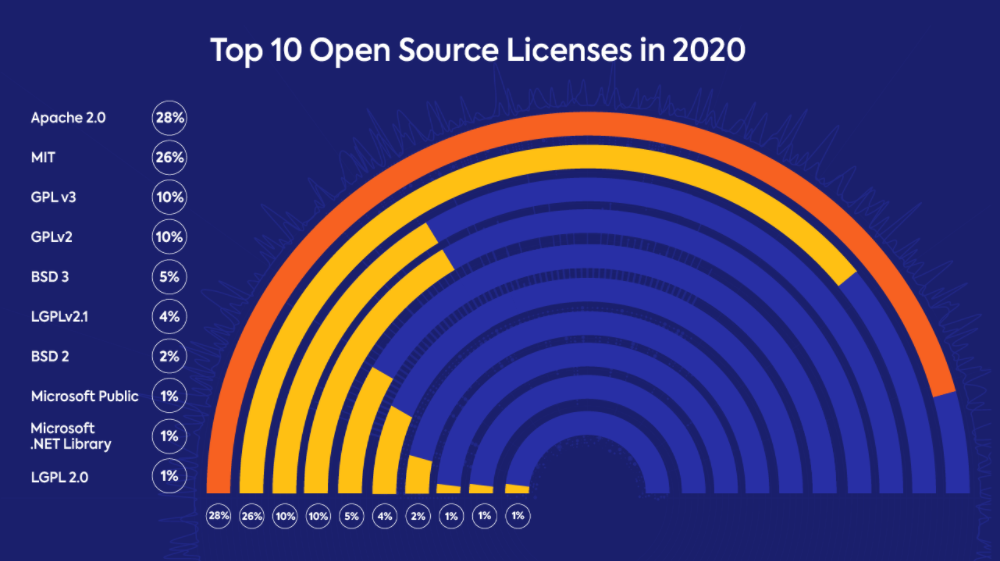
\includegraphics[scale=0.35]{Bilder/Statistik Verwendung OSS.png}
    \caption{Statistik über die Verwendung von OS-Lizenzen im Jahr 2020, (Quelle)}
\end{figure}

Anhand der Abbildung 10 wird der deutlich, welche OS-Lizenzen im Jahr 2020 am häufigsten genommen wurden. Trotz der hohen Verwendung von der Apache Licence 2.0, liegt die GNU 3.0 die ein starkes Copyleft aufweist, unter den oberen Plätzen. Gründe dafür sind, dass Entwickler, die ihre Projekte veröffentlichen an jeder Weiterentwicklung beteiligt sein möchten, was das Ziel der FSI ausmacht. 

\paragraph{2.2.4.1. Arten der OSS-Lizenzen} $~$

Im Folgenden wird ein kurzer Üblick über die wesentlichen Lizenzen erstellt. Aufgrund der hohen Anzahl an Lizenzen im Bereich der OSS, werden nur diejenigen vorgestellt, die innerhalb dieser Arbeit von Bedeutung sind und aktiv von der msg systems ag eingesetzt werden. 

\begin{itemize}
    \item Apache Licence 2.0 (Apache Lizenz)
    \item BSD-X-Clause (Berkeley Software Destribution Lizenzen 2-Clause/3-Clause)
    \item EPL 2.0 (Eclipse Public License 2.0)
    \item EUPL 1.2 (European Union Public License 1.2)
    \item CDDL 1.1 (Common Development and Distribution License 1.1)
    \item LGPL 3.0 (GNU Lesser General Public License 3.0)
    \item MIT (Massachusetts Institute of Technology Lizenz)
    \item MPL 2.0 (Mozilla Public License 2.0)
    \item GPL 3.0 (GNU General Public License 3.0)
\end{itemize}

\paragraph{2.2.4.2. Klassifizierung anhand des Copyleft-Statuses}$~$

Obwohl bei allen OSS-Lizenzen die Möglichkeit des freien Zugang zum Quellcode, der Veränderung, der Analyse und Weitergabe der modifizierten Software besteht, kann anhand des Copyleft-Effekts das Nutzungsrecht erheblich beeinflusst werden. Je nach Lizenz werden unterschiedliche Nutzungsrechte eingeräumt, wobei  unterschiedliche Plichten, insbesondere im Hinblick auf eine Modifikation und Weiterverbreitung erfüllt werden müssen. Die Basis der Klassifizierung der bestehenden Lizenzen erfolgt anhand der Stärke der Copyleft-Klauseln und ist in Abbildung 11 kategorisch dargestellt.

\subparagraph{OSS-Lizenzen ohne Copyleft}$~$

OSS-Lizenzen mit keinem Copyleft bilden die erste Klassifizierungsstufe ab. Dem Nutzer werden im Gegensatz zu Lizenzen mit starkem oder beschränktem Copyleft übergreifende Nutzungsrechte überlassen. Insbesondere im Hinblick auf die Weitergabe des Quellcodes darf der Nutzer selbst entscheiden ob er  Modifikationen an seiner Software als eine neue Software veröffentlicht. Der Nutzer hat dementsprechend das Recht, das Ergebnis seiner Arbeit für sich zu behalten, obwohl dieser eine freie Softwarebasis ursprünglich verwendet hat. (Quelle) Ferner hat der Nutzer die Möglichkeit, die veränderte Software als eine Closed-Software zu verteiben.(Quelle) Als ein bekanntes und als die weit verbreiteste Lizenz gilt die Apache Licence 2.0, die von der Apache Software Foundation (Quelle) enwickelt worden ist. Neben der Apache Licence gilt die Massachusetts Institute of Technology Lizenz (kurz: MIT) (Quelle) ebenfalls als eine bekannte Lizenz ohne Copyleft. Der Unterschied zu Apache besteht darin, dass der Lizenznehmer dazu verpflichtet ist, die Lizenzbestimmungen als auch den Urheberrechtsvermerk bei einer Weitergabe beizufügen. 

\subparagraph{OSS-Lizenzen mit beschränktem Copyleft}$~$

Grundsätzlich müssen OSS-Lizenzen, die ein beschränktes Copyleft aufweisen, Veränderungen oder Verbesserungen, immer unter derselben Lizenz weitergeben, wie zu dem Zeitpunkt wo der Nutzer die Ausgangssoftware erhalten hat. (Quelle) Daher ist der Nutzer verpflichtet, alle Modifikationen basierend auf der Ausgangssoftware als einen Quellcode für die Allgemeinheit zugänglich zumachen und diese ebenfalls unter dieselbe Lizenz mit beschränktem Copyleft zu veröffentlichen. Allerdings gibt es Abstufungen, da im Allgemeinen der Fokus dieser Art von Lizensierung im Bereich der Softwarebibliotheken dar und einen Zugriff oder eine statische/dynamische Verlinkung auf Bibliotheken ermöglicht. In diesem Fall werden zwei Fälle voneinander unterschieden. Verlinken Programme Bibliotheken die unter ein beschränktes Copyleft fallen und können unabhängig von ihnen vertrieben werden, so muss die veränderte Software nicht unter einem beschränktem Copyleft veröffentlicht werden, sondern kann eine andere Lizenz annehmen. (Quelle) Besteht jedoch eine Abhängigkeit zwischen der zugriffenen Bibliothek und dem Programm, wird dies als ein neues Werk angesehen und muss demgemäß unter die Lizenz der Ausgangssoftware weitergegeben werden. Demnach ist eine Verwendung von Lizenzen mit beschränktem Copyleft auch für kommerzielle Produkte möglich, basierend auf Tatsache, dass keine Modifikationen an der ursprünglichen Software durchgeführt werden.(Quelle) Diese Art der Ausdehnung stellt den wesentlichen Unterschied zu Lizenzen mit einem starken Copyleft dar. Das bekannteste Bespiel einer Lizenz mit einem schwachen Copyleft, stellt die GNU Lesser General Public License (kurz: LGPL) als die 'abgeschwächtere' Form der GPL dar. 

\subparagraph{OSS-Lizenzen mit starkem Copyleft}$~$

Innerhalb der OSS-Lizenzen, die mit einem starkem Copyleft lizensiert sind, müssen alle Veränderungen und Verbesserungen unter den gleichen Rahmenbedingungen genutzt und weitergegeben werden, zu dem Zeitpunkt wo der Nutzer die Ausgangssoftware erhalten hat. Die entsprechenden Veränderungen schließen alle Modifikationen der ursprünglichen Software als auch die Entwicklungen, die auf der Originalsoftware aufbauen, ein. (Quelle) Die Plicht des Nutzers ist es, alle Veränderungen basierend auf der ursprünglichen Software als einen Quellcode für die Allgemeinheit zugänglich zu machen und diese ebenfalls unter denselben Copyleft-Klauseln zu veröffentlichen. Als bekannteste und zudem heutzutage eine der weit verbreitesten Lizenzen mit starkem Copyleft gilt die GNU General Public License (kurz: GPL). Die GPL wurde durch Richard Stallman geprägt und erfüllt die oben genannte Kriterien einer OS-Lizensierung. (Quelle) Durch die Kerneigenschaft der GPL, Veränderungen ebenfalls durch die GPL zu lizensieren, ist es Nutzern nicht möglich, Teile einer GPL-Software in kommerziellen Produkten zu verwenden. (Quelle) Die GPL verfolgt mit der lizensierten Veröffentlichung das Ziel, dass modifizierte und verbesserte Versionen einer Software den Urhebern immer zur Verfügung stehen müssen. Darüber hinaus muss festgehalten werden, dass sich die Einschränkungen der GPL auf die Weiterverbreitung fokussiert. So ist Nutzern durchaus möglich, GPL-lizensierte Software intern zu verwenden ohne diese zu veröffentlichen. Basierend auf der GPL und LGPL wird das Zusammenspiel zwischen freier Software und OSS verdeutlich, indem der bestehende Lizneztext nach den Bedürfnissen einer großen Gemeinschaft angepasst wird und den Status einer neuen Lizenz erhält. (Quelle)

\begin{figure}[h]
    \centering
    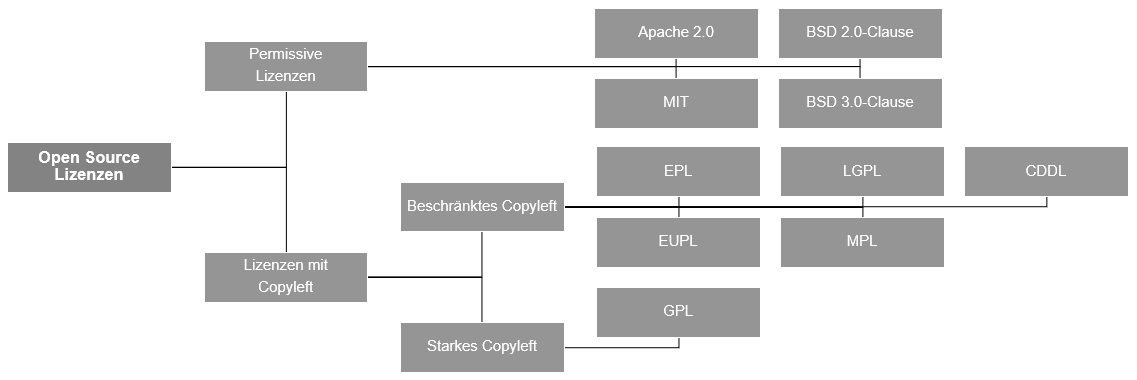
\includegraphics[scale=0.55]{Bilder/Lizenzenvarianten.png}
    \caption{OS-Lizenzen nach dem Status der dazugehörigen Copyleft-Klauseln}
\end{figure}

\paragraph{2.2.4.3. Rechte und Pflichten des Lizenznehmers basierend auf dem Copyleft-Status}$~$

Innerhalb der OSS-Lizenzen existieren erhebliche Unterschiede, die anhand der Rechte und Pflichten der jeweiligen Copyleft-Klauseln erkennbar sind und im nächsten Abschnitt näher ausgeführt werden. 

\subparagraph{Rechte des Lizenznehmers bei einer Lizenz mit keinem Copyleft}$~$

Grundsätzlich wird jedem Nutzer einer Lizenz mit keinem Copyleft, ein Nutzungsrecht eingeräumt. Demnach erhält der Nutzer das Recht auf die Veränderung, die Vervielfältigung als auch den Vertrieb von modifizierter und nicht-modifizierter Software. (Quelle) Darüber hinaus hat der Nutzer das Recht, die Software unter eigenen Lizenzbedingungen zu vertreiben oder diese proprietär lizensieren zu lassen, sodass eine Offenlegung des Quellcodes nicht mehr möglich ist.

\subparagraph{Rechte des Lizenznehmers bei einer Lizenz mit beschränktem Copyleft}$~$

Ähnlich wie bei Lizenzen mit keinem Copyleft, hat der Nutzer das Recht auf die Bearbeitung, die Vervielfältigung, die Weitergabe unveränderter und veränderter Software und die Nutzung für jegliche Zwecke der ursprünglichen Software. (Quelle) Zudem erfolgt die Weitergabe ohne zu errichteten Lizenzgebühren. Ein Beispiel für Nutzungsrechte innerhalb dieser Art von Copyleft, stellt die LGPL als die Tochter-Lizenz der GPL dar. (Quelle) Obwohl die LGPL 2.0 und GPL 2.0/3.0 miteinander kompatibel sind, legt die LGPL 3.0 fest, dass unter bestimmten Voraussetzungen das modifizierte Programm ausschließlich unter der GPL lizensiert werden kann. Die Folge ist, das aufgrund einer Weiterverbreitung von modifizierter Software und der entsprechenden Lizensierung von LGPL ausschließlich 2.0 verwendet werden darf und nicht mehr LGPL 3.0, die unter der GPL mit starkem Copyleft steht. (Quelle) Darüber hinaus hat der Nutzer das Recht, Bibliotheken in diesem Rahmen zu verändern und zu verbreiten. 

\subparagraph{Rechte des Lizenznehmers bei einer Lizenz mit starker Copyleft}$~$

Zunächst werden auch innerhalb der Lizenzen mit einem starken Copyleft, umfassende Nutzungsrechte eingeräumt. Wie auch bei jeder OS-Lizenz hat der Nutzer das Recht auf auf die Bearbeitung, die Vervielfältigung, die Weitergabe unveränderter und veränderter Software und die Nutzung für jegliche Zwecke der ursprünglichen Software. (Quelle) Auch hier erfolgt die Weitergabe ohne die Errichtung von Lizenzgebühren. Folglich besitzt jeder Nutzer die Möglichkeit auf Weiterentwicklung der lizensierten Software. Darüber hinaus darf unter der GPL 2.0 und 3.0 unveränderte Kopien des Quellcodes zu erstellen und diese für die Allgemeinheit zugänglich zu machen und zu verbreiten. (Quelle)

\subparagraph{Pflichten des Lizenznehmers bei einer Lizenz mit keinem Copyleft}$~$

Die Lizenzbedingungen ohne Copyleft-Effekt enthalten kaum Pflichten für den Nutzer als es bei einer Lizenz mit beschränkter oder starker Copyleft der Fall ist. (Quelle) Grundsätzlich muss der Nutzer die OS-Lizenz als ein Lizenztext bei der Weitergabe beifügen. Der Lizenztext sollte neben den Lizenzbestimmungen, der Urheber- und der Copyright-Vermerk und den Haftungs- und Gewährleistungsanspruch beinhalten. Trotz des Copylefts können je nach Lizenz unterschiedliche Bedingungen erfüllt werden. So muss bei der Weitergabe der Modifikationen gemäß der Berkeley Software Destribution (kurz: BSD) keine Autorenhinweise bestehen, während dies von der Apache Licence zwingend vorausgesetzt wird. (Quelle) Darüber hinaus unterscheidet die BSD Software nach ihren Modifikationen. So müssen modifizierte oder neue Bestandteile die aufgeführten Pflichten nicht erfüllen, während für unveränderte bestehende Komponenten, dies tun müssen. (Quelle) Auch hier findet sich ein wesentlicher Unterschied zu der Apache Licence, da hierbei die Software als Ganzes und ohne eine Abspaltung zwischen modifizierter und bestehender Komponeten betrachetet wird. 

\subparagraph{Pflichten des Lizenznehmers bei einer Lizenz mit beschränktem Copyleft}$~$

Wesentliche allgemeine Pflichten des Nutzers bestehen darin, die Lizenz als einen Lizenztext weiterzugeben, den Copyrightvermerk beizubehalten und einen Haftungsausschuss festzuhalten. (Quelle) Zudem müssen beispielweise bei der LGPL 3.0 hinsichtlich der Pflichten unterschieden werden, ob die Weitergabe sich auf eine geänderte oder um eine unveränderte Software bezieht. Sobald bei einer Software ausschließlich die Bibliothek an sich verändert worden ist ("work based on the libary"), greift der Copyleft-Effekt und die modifizierte Software muss unter dieselbe Lizenz veröffentlicht werden wie die Ausgangssoftware. (Quelle) Wird allerdings die Software verändert, die die Bibliothek verlinkt ("work that uses the libary"), kann die Weitergabe der Software unter einer anderen Lizenz erfolgen und es erfolgt eine Abweichnung des starken Copylefts. (Quelle) Ferner können Bibliotheken unter der LGPL 3.0 in Kombination mit proprietären Programmen verwendet werden.(Quelle) 

\subparagraph{Pflichten des Lizenznehmers bei einer Lizenz mit starker Copyleft}$~$

Die Pflichten des Lizenznehmers bei einer Lizenz mit starker Copyleft, sind im Vergleich zu Lizenzen mit keinem Copyleft um ein vielfaches ausgeprägter. Sobald der Nutzer die entsprechende veränderte Software im Rahmen der starken Copyleft-Klauseln weitergeben möchte, muss dieser umfassende Pflichten (3xQuelle) berücksichtigen: 

\begin{itemize}
    \item Zugänglicher Quellcode\\
    Wird die modifizierte Software vertrieben, muss der Nutzer sicherstellen, dass der Quellcode jederzeit und für jedermann frei zugänglich ist. Zum Quellcode gehören alle Quelltexte, die kompiliert werden müssen sowie alle Skripte und Dateien für die Implementierung der Schnittstellen. So bietet die GPL, zwei Optionen für die Sicherstellung des freien Zugangs an. (Quelle) Im ersten Fall ist der Nutzer verpflichtet, den Quellcode auf einem Datenträger beizufügen. Diese Option wird in der GPL 3.0 nicht mehr vorgegeben, da sie nicht mehr zeitkonform ist, sodass das Angebot eines kostenlosen Downloads für diesen Zweck ausreicht. Die andere Option beschreibt ein Angebot zur Lieferung des Quellcodes innerhalb drei Jahren an jeden Dritten, wodurch jeder den Anspruch erhält, die Software für sich zu nutzen. Bei der GPL 3.0 ist der Nutzer verpflichtet, den Quellcode bereitzustellen, wie er die Lieferung für die Software anbietet, wodurch eine zeitliche Vorgabe entfällt.  

    \item Vertrieb von veränderter Software basierend auf dem Copyleft\\
    Im Gegensatz zu Lizenzen mit keinem Copyleft, verpflichtet sich der Nutzer bei Lizenzen mit starker Copyleft dazu, die modifizierte Software unter der gleichen OS-Lizenz weiterzugeben wie die urspüngliche Software dem Nutzer überlassen worden ist. (Quelle) Damit soll die Weiterentwicklung des ursprünglichen Programmes sichergestellt und die Rechte des Urhebers geschützt werden. Ab wann eine derartige Modifikation vorliegt, kann insbesondere aus der GPL 2.0 und 3.0 nicht bestimmt werden. Allerdings beschränkt sich die Verpflichtung nicht auf die Weitergabe der eigentlichen Modifikation, sondern auf die modifizierte Software als Ganzes. (Quelle) 

    \item Verbot der Lizenzgebühren\\
    Ein wesentlicher Kernaspekt der OS-Lizenzen darin besteht, Software ohne die Errichtung von Lizenzgebühren für alle frei zugänglich zu machen. Dies ist in der GPL 2.0 nur indirekt verankert, indem lediglich darauf hingewiesen wird, dass keine Gewährleistung übernommen wird, da für die Software keine Lizenzgebühren zu errichten sind. (Quelle) Innerhalb der GPL 3.0 besteht die Verpflichtung, dass bei einer Weitergabe keine Lizenzkosten zu errichten sind. 

    \item Vorhandensein des Lizenztextes\\
    Zunächst muss der vollständige Lizenztext bei der Weitergabe der Software beigelegt werden. Häufig wird hier eine seperate Datei erstellt, wo sich der betreffende Lizenztext befindet, damit es für den Nutzer eindeutig erkennbar ist, welche Komponenten oder Programme eine Lizenz mit starker Copyleft aufweisen. (Quelle) 

    \item Urhebervermerk\\
    Des Weiteren ist der Nutzer hinsichtlich einer Vervielfältigung durch Kopien oder Vertreibung der Software verpflichtet, die Copyright und Urherber-Vermerke beizufügen und zu veröffentlichen. (Quelle) Um die Veränderungen nachvollzuziehen zu können, muss bei der Verteilung von veränderter Software ein Hinweis auf die Modifikation und deren Datum vorliegen. 
    
    \item Haftungsausschuss\\
    Ferner ist der Nutzer verpflichtet, einen Haftungsausschuss bei der Weitergabe von veränderter Software, für jeden klar erkennbar, beizufügen, ohne bereits vorhandene Haftungsausschüsse zu entfernen. (Quelle) Grundsätzlich ist der Vermerk nach einem Haftungsausschuss nach deutschem Recht nicht gültig, allerdings sollte dieses beibehalten werden, da Ansprüche Dritter gegen das Unternehmen aus dem Ausland möglich sind und damit abgefangen werden können.  

    \item Abweichende Vereinbarungen\\
    Gemäß der GPL 2.0 ist es nicht gestattet, Beschränkungen innerhalb des Lizenztext hinzufügen oder die Verteilung der Software anhand zusätzlicher Pflichten abhängig zu machen. (Quelle)  Innerhalb der GPL 3.0 wurden einerseits die 'Additional permissions' hinzugefügt, die die Ergänzung und die Befreiung von zusätzlichen Lizenzpflichten regeln und anderseits eine Liste mit zusätzlichen Beschränkungen hinzugefügt, die die Bedingungen von anzugebenden unbekannten Pflichten in der GPL regeln. Damit verfolgt die GPL 3.0 das Ziel, die Möglichkeit der Intergration des Quellcodes mit abweichenden Lizenzen zu erleichtern und die Kompabilität zu anderen Lizenzen zu erweitern. (Quelle)     
\end{itemize}

\paragraph{2.2.4.4. Kompabilität der OSS-Lizenzen}$~$

Müssen unterschiedliche Komponenten einer Software gemeinsam genutzt oder im Rahmen eines gesamten Produkts miteinander kombiniert und weitergegeben werden, so muss die Kompabilität der einzelnen Lizenzen anhand der Softwarekomponenten berücksichtigt werden. (Quelle) Die Kompabilität wird in der Regel als eine Öffnungs- oder Kompabilitätsklausel in den Lizenzbestimmungen festgelegt. (Quelle) Eine mögliche Inkompabiliät ist gegeben, wenn das Produkt mit mindestens zwei, sich im Widerspruch stehenden Lizenzen vertrieben werden. (Quelle)\\\\ Zunächst muss überprüft werden, ob eine Kompabilität der Softwarekomponenten ohne und mit Copyleft besteht. Sollte eine Komponente eine Lizenz mit einer starken Copyleft-Klausel beinhalten, muss deren Kompabilität untersucht werden. Diese Überprüfung ist essentiell, da Softwarekomponenten mit starken Copyleft-Klauseln die Lizenzbedingung beinhalten, dass modifizierte Software unter den gleichen Bedingungen vertrieben wird wie die Ausgangssoftware. Insbesondere die GPL schließt Kompabilitätsklauseln von vornherein aus, da die modifizierte Software ausschließlich unter ihrer eigenen Lizenz weiterverbeitet werden soll. Allerdings wurden durch die GPL 3.0 die Additional permissions und die Liste der zusätzlichen Beschränkungen veröffentlicht, die eine Kompabilität in bestimmten Fällen erlauben. (Quelle) Sollten mehrere Softwarekomponenten mit Lizenzen ohne Copyleft abhängig miteinander funktionieren, liegt keine Inkompabiliät vor. Die LGPL weist in dieser Hinsicht, eine Kompabilität nur unter bestimmten Voraussetzungen insbesondere anhand einer statischen oder dynamischen Verlinkung voraus. Dementsprechend muss zunächst geprüft werden, ob die Funktionalität mehrerer Komponenten unabhängig voneinander oder abhängig miteinander gewährleistet wird. Sollte eine Softwarekomponente ein beschränktes Copyleft aufweisen und ausschließlich mit anderen Komponenten miteinander funktionieren, muss die Kompabilität geprüft werden, da diese im Zweifelsfall unter dieser Lizenz weiterverbreitet werden müssen. (Quelle) Werden Softwarekomponenten mit beschränktem Copyleft-Klauseln miteinander genutzt, wobei die originalen Komponenten unabhängig voneinander funktionieren, kann die Kompabilität sichergestellt werden. (Quelle) \\\\ Darüber hinaus dürfen keine Lizenzbedingungen enthalten sein, die der ursprüngliche Lizenz nicht bekannt ist. (Quelle) Insbesondere Softwarekomponenten ohne Copyleft weisen Bedingungen auf, die beispielweise die die GPL nicht kennt und daher zu einer Inkompabiliät führt. Auch aufgrund der Tatsache, dass Unternehmen heutzutage dazu tendieren, Lizenzen von Softwarekomponenten ohne Copyleft zu verwenden wie in Abbildung 10 dargestellt, da diese im Vergleich zu anderen Lizenzen wesentlich flexibler sind, sollte diese Überprüfung durchgeführt werden. 

\begin{figure}[h]
    \centering
    \includegraphics[scale=0.55]{Bilder/Kompatibilität.png}
    \caption{Kompabilität der OS-Lizenzen, angelehnt an (Quelle)}
\end{figure}

Anhand der vorliegenden Abbildung 12 wird die Kompabilität der unterschiedlichen Lizenzen visuell dargestellt. Die Pfeile zeigen an, dass eine Modifikation zu der dazugehörigen Lizenz möglich ist. Eine wesentliche Besonderheit zeigt die Inkompabiliät zwischen GPL und LGPL. (Quelle) So besteht eine Kompabilität zwischen LGPL 2.1 only und GPL 2.0 und 2.0 only, jedoch nicht zu LGPL 3.0. Auch GPL 2.0 und GPL 3.0 sind eigentlich nicht kompatibel zueinander, wobei in beiden Lizenzen die Bedingungen angegeben ist, dass letztlich der Lizenzgeber entscheiden kann, welche Version der GPL er nehmen kann und daher von Kompatibilität ausgegangen werden kann. (Quelle) Auch die GPL 3.0 und die GPL 2.0 only sind aufgrund des Copyleft-Effekts beideer Lizenzen nicht miteinander kompatibel. 














